% SAMPLE-ONLY: \SampleGuideNote and \SampleGuideSource are not template commands.
\section{実験方法}
\label{sec:method}

\subsection{使用機器}
\label{subsec:equipment}

% [DOC:LIST-BASIC-01] Basic LaTeX list with explicit lengths.
使用機器と素子を以下に示す。
\begin{list}{--}{%
  \setlength{\leftmargin}{2.8em}%
  \setlength{\itemsep}{0.15em}%
  \setlength{\parsep}{0pt}%
}
  \item 信号発生器：Sample Generator A
  \item オシロスコープ：Sample Scope B
  \item デジタルマルチメータ：Sample Meter C
  \item 10 倍受動プローブ：2 本
  \item 金属皮膜抵抗：公称値 \qty{1.00}{\kilo\ohm}
  \item フィルムコンデンサ：公称値 \qty{0.100}{\micro\farad}
  \item ブレッドボード、接続線、BNC 変換端子
\end{list}

\SampleGuideNote[teal!70!black]{［LIST-BASIC-01］}{%
LaTeX の基本 \texttt{list} 環境では、第 1 引数にラベル、第 2 引数に余白や項目間隔を記述できます。}

各機器の主な設定と用途を\cref{tab:equipment}に示す。機器の仕様は、
校正記録と公開資料を参照して整理した\cite{jp-report,jp-online,jp-misc}。

% [DOC:TABLE-TABULARX-01] Instrument table with an X column.
% guide_equipment_table_start
\begin{table}[htbp]
  \centering
  \caption{使用機器の設定と用途}
  \label{tab:equipment}
  \begin{tabularx}{\linewidth}{
      >{\raggedright\arraybackslash}p{0.20\linewidth}
      >{\raggedright\arraybackslash}p{0.22\linewidth}
      >{\raggedright\arraybackslash}X}
    \toprule
    機器 & 主な設定 & 本実験での用途 \\
    \midrule
    信号発生器
      & 正弦波、\qty{1.00}{\volt}、出力抵抗 \qty{50}{\ohm}
      & \qty{100}{\hertz} から \qty{10}{\kilo\hertz} まで周波数を変化させ、RC 回路へ一定振幅の信号を入力する。\\
    オシロスコープ
      & 2 チャンネル、AC 結合、時間差カーソル
      & 入力波形と出力波形を同時に表示し、振幅と二つの波形の時間差を読み取る。\\
    デジタルマルチメータ
      & 抵抗測定、容量測定
      & 回路を構成する前に抵抗値と静電容量を三回ずつ測定する。\\
    10 倍プローブ
      & 入力容量 \qty{12}{\pico\farad}、入力抵抗 \qty{10}{\mega\ohm}
      & 回路への負荷を小さくしながら、入力側と出力側の電圧を測定する。\\
    \bottomrule
  \end{tabularx}
\end{table}
% guide_equipment_table_end

\SampleGuideSource
  {幅に合わせて文章を折り返す表のコード}
  {sections/03-method.tex}
  {guide_equipment_table_start}
  {guide_equipment_table_end}

\SampleGuideNote[orange!80!black]{［TABLE-TABULARX-01］}{%
\texttt{tabularx} の \texttt{X} 列は、表の残った幅を使います。
文章が長い場合は、列の中で自動的に折り返されます。}

\SampleGuideNote[orange!80!black]{固定幅列の補足}{%
最初の二列には折り返し可能な \texttt{p} 列を使い、機器名と設定の列幅を固定しています。}

\subsection{素子値の予備測定}
\label{subsec:component-measurement}

抵抗とコンデンサを回路へ取り付ける前に、それぞれ三回測定した。
端子に触れないように部品を固定し、測定値が安定してから記録した。
結果を\cref{tab:components}に示す。

% [DOC:TABLE-PCOLUMN-01] Fixed-width wrapping columns.
\begin{table}[H]
  \centering
  \caption{素子値の予備測定結果}
  \label{tab:components}
  \setlength{\tabcolsep}{3pt}
  \begin{tabularx}{\linewidth}{
      >{\centering\arraybackslash}p{0.13\linewidth}
      >{\centering\arraybackslash}p{0.11\linewidth}
      >{\centering\arraybackslash}p{0.11\linewidth}
      >{\centering\arraybackslash}p{0.11\linewidth}
      >{\centering\arraybackslash}p{0.11\linewidth}
      >{\raggedright\arraybackslash}X}
    \toprule
    素子 & 1 回目 & 2 回目 & 3 回目 & 平均値 & 測定時の状態 \\
    \midrule
    抵抗
      & \qty{0.998}{\kilo\ohm}
      & \qty{0.999}{\kilo\ohm}
      & \qty{0.998}{\kilo\ohm}
      & \qty{0.998}{\kilo\ohm}
      & 端子間を直接測定し、周囲温度は \qty{24}{\degreeCelsius} であった。\\
    コンデンサ
      & \qty{0.101}{\micro\farad}
      & \qty{0.101}{\micro\farad}
      & \qty{0.100}{\micro\farad}
      & \qty{0.101}{\micro\farad}
      & 測定前に端子を短絡して残留電荷を除いた。\\
    \bottomrule
  \end{tabularx}
\end{table}

\SampleGuideNote[orange!80!black]{［TABLE-PCOLUMN-01］}{%
数値列には固定幅の \texttt{p} 列を使い、狭い列の中でも内容を自動的に折り返しています。}

% [DOC:TABLE-BOOKTABS-01] Top, middle, and bottom rules.
\SampleGuideNote[orange!80!black]{［TABLE-BOOKTABS-01］}{%
\texttt{booktabs} の \texttt{\string\toprule}、\texttt{\string\midrule}、
  \texttt{\string\bottomrule} で表の横罫線を整理しています。}

% [DOC:FLOAT-H-01] Exact float placement from the float package.
\SampleGuideNote[orange!80!black]{配置の補足}{%
この表は測定方法の直後に置くため、\texttt{float} が提供する位置指定 \texttt{[H]} を使用しています。}

\subsection{回路と測定装置}
\label{subsec:apparatus}

% [DOC:DIAG-CIRCUIT-01] CircuitikZ RC circuit.
% [DOC:DIAG-APPARATUS-01] TikZ apparatus diagram.
% [DOC:DIAG-FRAME-01] mdframed around the apparatus.
\begin{figure}[H]
  \centering
  \begin{subfigure}[t]{0.47\linewidth}
    \centering
    \begin{circuitikz}[american voltages]
      % guide_circuit_start
      \draw
        (0,0) node[left]{$V_{\mathrm{in}}$}
        to[R,l=$R$] (2.4,0)
        -- (3.3,0) node[right]{$V_{\mathrm{out}}$}
        (2.4,0) to[C,l=$C$] (2.4,-2)
        -- (0,-2) -- (0,0);
      % guide_circuit_end
    \end{circuitikz}
    \caption{RC 低域通過回路}
    \label{fig:rc-circuit}
  \end{subfigure}
  \hfill
  \begin{subfigure}[t]{0.47\linewidth}
    \centering
    \begin{mdframed}[
      linecolor=black!60,
      linewidth=0.7pt,
      roundcorner=3pt,
      innerleftmargin=3pt,
      innerrightmargin=3pt,
      innertopmargin=5pt,
      innerbottommargin=5pt
    ]
      \centering
      \begin{tikzpicture}[
        device/.style={draw,rounded corners,align=center,minimum width=15mm,minimum height=9mm,font=\small},
        >=Latex
      ]
        \node[device] (generator) {信号\\発生器};
        \node[device,right=4mm of generator] (filter) {RC\\回路};
        \node[device,right=4mm of filter] (scope) {オシロ\\スコープ};
        \draw[->] (generator) -- node[above,font=\scriptsize] {$V_{\mathrm{in}}$} (filter);
        \draw[->] (filter) -- node[above,font=\scriptsize] {$V_{\mathrm{out}}$} (scope);
        \coordinate (groundmid) at ($(generator.south)!0.5!(scope.south)$);
        \draw (generator.south) -- ++(0,-5mm) -| (scope.south);
        \node[below=1mm of groundmid,font=\scriptsize] {共通 GND};
      \end{tikzpicture}
    \end{mdframed}
    \caption{測定装置の接続}
    \label{fig:apparatus}
  \end{subfigure}
  \caption{RC 回路と測定装置}
  \label{fig:method-overview}
\end{figure}

\SampleGuideSource
  {RC 回路を描いている部分}
  {sections/03-method.tex}
  {guide_circuit_start}
  {guide_circuit_end}

\Cref{fig:method-overview}に回路と装置の接続を示す。
信号発生器の出力を抵抗へ接続し、コンデンサ両端を出力とした。
オシロスコープの CH1 で入力電圧、CH2 で出力電圧を同時に測定した。
回路構成と装置接続の詳細は\crefrange{fig:rc-circuit}{fig:apparatus}に分けて示している。

\SampleGuideNote[orange!80!black]{［DIAG-CIRCUIT-01］}{%
\cref{fig:rc-circuit}は \texttt{circuitikz} の抵抗素子とコンデンサ素子を接続して描いています。}

% [DOC:DIAG-TIKZ-01] TikZ nodes, relative positioning, and arrows.
\SampleGuideNote[orange!80!black]{［DIAG-TIKZ-01］}{%
\cref{fig:apparatus}の装置は TikZ の \texttt{positioning} で相対配置し、
  \texttt{arrows.meta} の矢印で信号方向を示しています。}

% [DOC:DIAG-CALC-01] Coordinate calculation with the TikZ calc library.
\SampleGuideNote[orange!80!black]{座標計算の補足}{%
共通 GND の文字位置は、\texttt{calc} を用いて信号発生器とオシロスコープの中点から求めています。}

\SampleGuideNote[orange!80!black]{［DIAG-FRAME-01］}{%
\texttt{mdframed} は注釈を囲むためではなく、ここでは測定装置全体を一つの枠線図として囲むために使用しています。}

% [DOC:FIG-SUBFIGURE-01] Two subfigures under one parent figure.
\SampleGuideNote[orange!80!black]{［FIG-SUBFIGURE-01］}{%
二つの \texttt{subfigure} を一つの \texttt{figure} に入れると、個別の小見出しと全体の図題を付けられます。}

% [DOC:REF-SUBFIG-RANGE-01] Range reference across two subfigures.
\SampleGuideNote[blue!65!black]{子図をまとめて参照する場合}{%
二つの子図のラベルを \texttt{\string\crefrange} に渡すと、子図番号を一つの範囲として表示できます。}

\subsection{測定許可の判定}
\label{subsec:trigger-logic}

自動記録を開始する条件として、CH1 の入力振幅が設定範囲内にあり、
CH2 の波形が安定していることの両方を確認した。
この判定を概念的な論理回路として\cref{fig:trigger-logic}に示す。

% [DOC:DIAG-LOGIC-01] US-style logic circuit.
\begin{figure}[htbp]
  \centering
  \begin{tikzpicture}[
    circuit logic US,
    every circuit symbol/.style={draw,fill=white},
    >=Latex
  ]
    \node (ch1) at (0,0.7) {CH1 振幅 OK};
    \node (ch2) at (0,-0.7) {CH2 波形安定};
    \node[and gate] (gate) at (4,0) {};
    \node[right=16mm of gate] (record) {記録開始};
    \draw[->] (ch1.east) -- ++(5mm,0) |- (gate.input 1);
    \draw[->] (ch2.east) -- ++(5mm,0) |- (gate.input 2);
    \draw[->] (gate.output) -- (record.west);
  \end{tikzpicture}
  \caption{測定許可条件の概念論理}
  \label{fig:trigger-logic}
\end{figure}

\SampleGuideNote[orange!80!black]{［DIAG-LOGIC-01］}{%
\texttt{circuits.logic.US} の \texttt{and gate} を使い、二つの条件が同時に成立する判定を描いています。}

\subsection{プローブ補償と波形確認}
\label{subsec:probe-calibration}

測定開始前に信号発生器とオシロスコープを \qty{10}{\minute} 動作させた。
プローブ倍率を両チャンネルとも 10 倍に設定し、校正端子の矩形波を用いて補償を調整した\cite{jp-incollection}。
その後、\qty{1.60}{\kilo\hertz} の正弦波を入力し、遮断周波数付近で
二つの波形が安定して表示されることを確認した。

% [DOC:FIG-IMAGE-01] External image inserted with graphicx.
% guide_image_start
\begin{figure}[H]
  \centering
  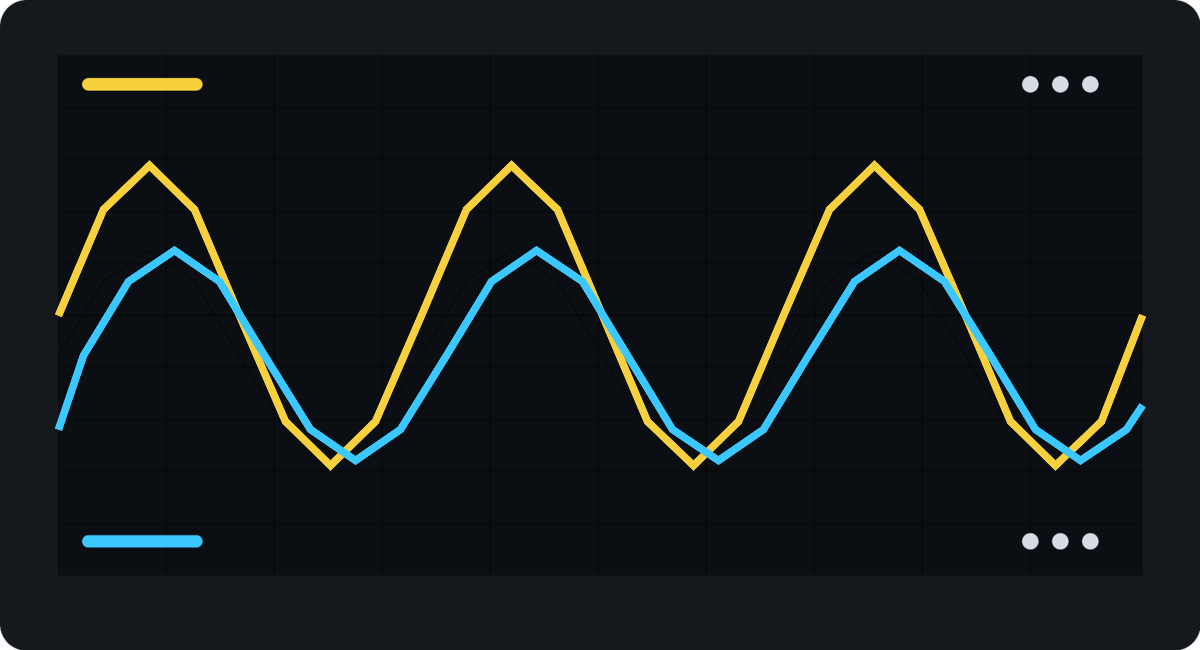
\includegraphics[width=0.82\linewidth]{oscilloscope-waveform.png}
  \caption{遮断周波数付近で観測した入力波形と出力波形}
  \label{fig:oscilloscope-waveform}
\end{figure}
% guide_image_end

\SampleGuideSource
  {外部画像を挿入するコード}
  {sections/03-method.tex}
  {guide_image_start}
  {guide_image_end}

\SampleGuideNote[orange!80!black]{［FIG-IMAGE-01］}{%
画像は \texttt{\string\includegraphics} で読み込みます。
ここでは \texttt{width=0.82\string\linewidth} とし、本文幅より少し小さく表示しています。}

\SampleGuideNote[orange!80!black]{画像パスの補足}{%
\texttt{report.tex} の \texttt{\string\graphicspath} により、ファイル名だけで \texttt{figures/} 内の画像を参照できます。}

% [DOC:LINK-HYPERREF-01] Hidden-border links for references and URLs.
\SampleGuideNote[orange!80!black]{ハイパーリンクの補足}{%
図番号や文献 URL には \texttt{hyperref} がリンクを付けますが、\texttt{hidelinks} により枠線は表示されません。}

\subsection{測定条件}
\label{subsec:conditions}

測定中に一定とする条件を以下に示す。

% [DOC:LIST-ITEMIZE-03] Measurement conditions.
\begin{itemize}[leftmargin=3em,itemsep=0.25em]
  \item 入力波形は正弦波とし、入力振幅は \qty{1.00}{\volt} に保つ。
  \item 周波数は低い側から高い側へ変化させ、遮断周波数付近では測定間隔を小さくする。
  \item 各周波数で振幅と時間差を三回読み取る。
  \item 周波数変更後は波形が安定してから記録する。
  \item 入力と出力のグラウンドは共通にする。
\end{itemize}

\SampleGuideNote[teal!70!black]{条件整理の補足}{%
同じ \texttt{itemize} 環境を、目的だけでなく測定中に固定する条件の整理にも使用できます。}

\subsection{測定手順}
\label{subsec:procedure}

% [DOC:LIST-ENUMERATE-01] Numbered measurement procedure.
測定手順は次のとおりとした。
% guide_enumerate_start
\begin{enumerate}[label=(\arabic*),leftmargin=3em,itemsep=0.25em]
  \item 抵抗値と静電容量を三回測定し、平均値を求める。
  \item \cref{fig:rc-circuit}の回路を構成し、配線を目視確認する。
  \item 信号発生器を正弦波、\qty{100}{\hertz}、\qty{1.00}{\volt} に設定する。
  \item CH1 と CH2 の零点、電圧軸および時間軸を調整する。
  \item \qty{100}{\hertz} から \qty{10}{\kilo\hertz} まで周波数を変化させ、振幅と時間差を記録する。
  \item \qtyrange{1.30}{2.00}{\kilo\hertz} では測定点を追加する。
  \item \qty{2.00}{\kilo\hertz} から \qty{500}{\hertz} まで逆方向にも測定し、走査方向の差を確認する。
  \item 測定終了後に入力を停止し、回路を取り外す。
\end{enumerate}
% guide_enumerate_end

\SampleGuideSource
  {番号付きの手順を書くコード}
  {sections/03-method.tex}
  {guide_enumerate_start}
  {guide_enumerate_end}

\SampleGuideNote[teal!70!black]{［LIST-ENUMERATE-01］}{%
順番が大切な手順には \texttt{enumerate} を使います。
\texttt{label=(\string\arabic*)} を付けると、番号を「(1)」の形にできます。}

\subsection{データの保存形式}
\label{subsec:data-format}

測定値は CSV ファイルへ保存した。各列の意味を以下に示す。

% [DOC:LIST-DESCRIPTION-03] Description list for CSV fields.
\begin{description}[leftmargin=12em,labelwidth=10.5em,nosep]
  \item[\texttt{frequency\_hz}] 入力周波数（\unit{\hertz}）
  \item[\texttt{gain\_measured}] 測定した利得（\unit{\decibel}）
  \item[\texttt{gain\_theory}] 素子値から計算した利得（\unit{\decibel}）
  \item[\texttt{phase\_measured}] 測定した位相差（\unit{\degree}）
  \item[\texttt{phase\_theory}] 理論式から計算した位相差（\unit{\degree}）
  \item[\texttt{residual\_db}] 測定利得と理論利得の差（\unit{\decibel}）
\end{description}

ファイル名は \lstinline|frequency-response.csv| とし、解析プログラムから同じ名前で読み込んだ。

% [DOC:CODE-INLINE-01] Inline code fragment.
\SampleGuideNote[red!65!black]{［CODE-INLINE-01］}{%
本文中の短いファイル名や変数名は、\texttt{listings} の \texttt{\string\lstinline} で等幅表示できます。}
